\paragraph{1. Library toevoegen}
Eerst moet de React Native Sensors library worden toegevoegd aan de root van ons project.
Deze wordt toegevoegd met volgende commando:
\begin{minted}{bash}
npm install react-native-sensors --save
\end{minted}

\paragraph{2. Package teruggeven}
Normaal gezien moet de package dan worden toegevoegd aan het 
\textit{android/app/src/} \textbf{main/java/com/project/MainApplication.java} bestand.
Maar dit is niet meer nodig bij React Native 0.60+.

\paragraph{3. gradle instellingen aanpassen}
Tot slot moet volgende regel worden toegevoegd aan het \textit{android/app/build.gradle} bestand.
\begin{minted}{groovy}
implementation project(':react-native-sensors')
\end{minted}
En moet volgende regel worden toegevoegd aan het \textit{android/settings.gradle} bestand.
\begin{minted}{groovy}
include ':react-native-sensors'
project(':react-native-sensors').projectDir = 
    new File(rootProject.projectDir
        , '../node_modules/react-native-sensors/android')
\end{minted}
De package is nu volledig geïnstalleerd en klaar voor gebruik.

\paragraph{4. Sensor gebruiken}
Eerst wordt de library in het bestand waar we deze nodig hebben geïmporteerd.
\begin{minted}{typescript}
import { accelerometer, gyroscope } from "react-native-sensors";
\end{minted}
Daarna worden twee variabelen die de data van de sensoren zal bewaren aangemaakt.
\begin{minted}{typescript}
const [accelerometerData, setAccelerometerData] = useState({});
const [gyroscopeData, setGyroscopeData] = useState({});
\end{minted}
Tot slot kunnen deze variabelen gebruikt worden om de data van de sensoren op te vangen.
\begin{minted}{typescript}
const getData = () => {
    setIsFetchingData(true);

    startFetchingData();
};

const startFetchingData = () => {
    if (isFetchingData) {
        const accelerometerSubscription = new Accelerometer({
            updateInterval: 100, // Verander dit indien nodig
        }).subscribe(({ x, y, z }) => {
            // Doe iets met de accelerometerwaarden (x, y, z)
        });

        const gyroscopeSubscription = new Gyroscope({
        updateInterval: 100, // Verander dit indien nodig
        }).subscribe(({ x, y, z }) => {
            // Doe iets met de accelerometerwaarden (x, y, z)
        });

        // Unsubscribe van de sensoren wanneer je klaar bent 
        // met het ophalen van de data
        return () => {
            accelerometerSubscription.unsubscribe();
            gyroscopeSubscription.unsubscribe();
        };
    }
};
\end{minted}

\paragraph{4. Applicatie maken}
Net zoals bij de native applicatie wordt een applicatie gemaakt die de accelerometer en gyroscoop data 
opvraagt en weergeeft. Deze bestaat uit twee \textbf{<Text>} componenten voor de data van de
accelerometer en gyroscoop weer te geven en tot slot twee \textbf{<Button>} componenten om de 
data op te halen. Als de knoppen ingedrukt worden, dan wordt ofwel de
\textbf{getAccelerometerData} of \textbf{getGyroscopeData} methode aangeroepen. In deze methodes wordt de data 
van de sensoren opgehaald en in de \textbf{<Text>} componenten geplaatst.
\begin{figure}[H]
    \centering
    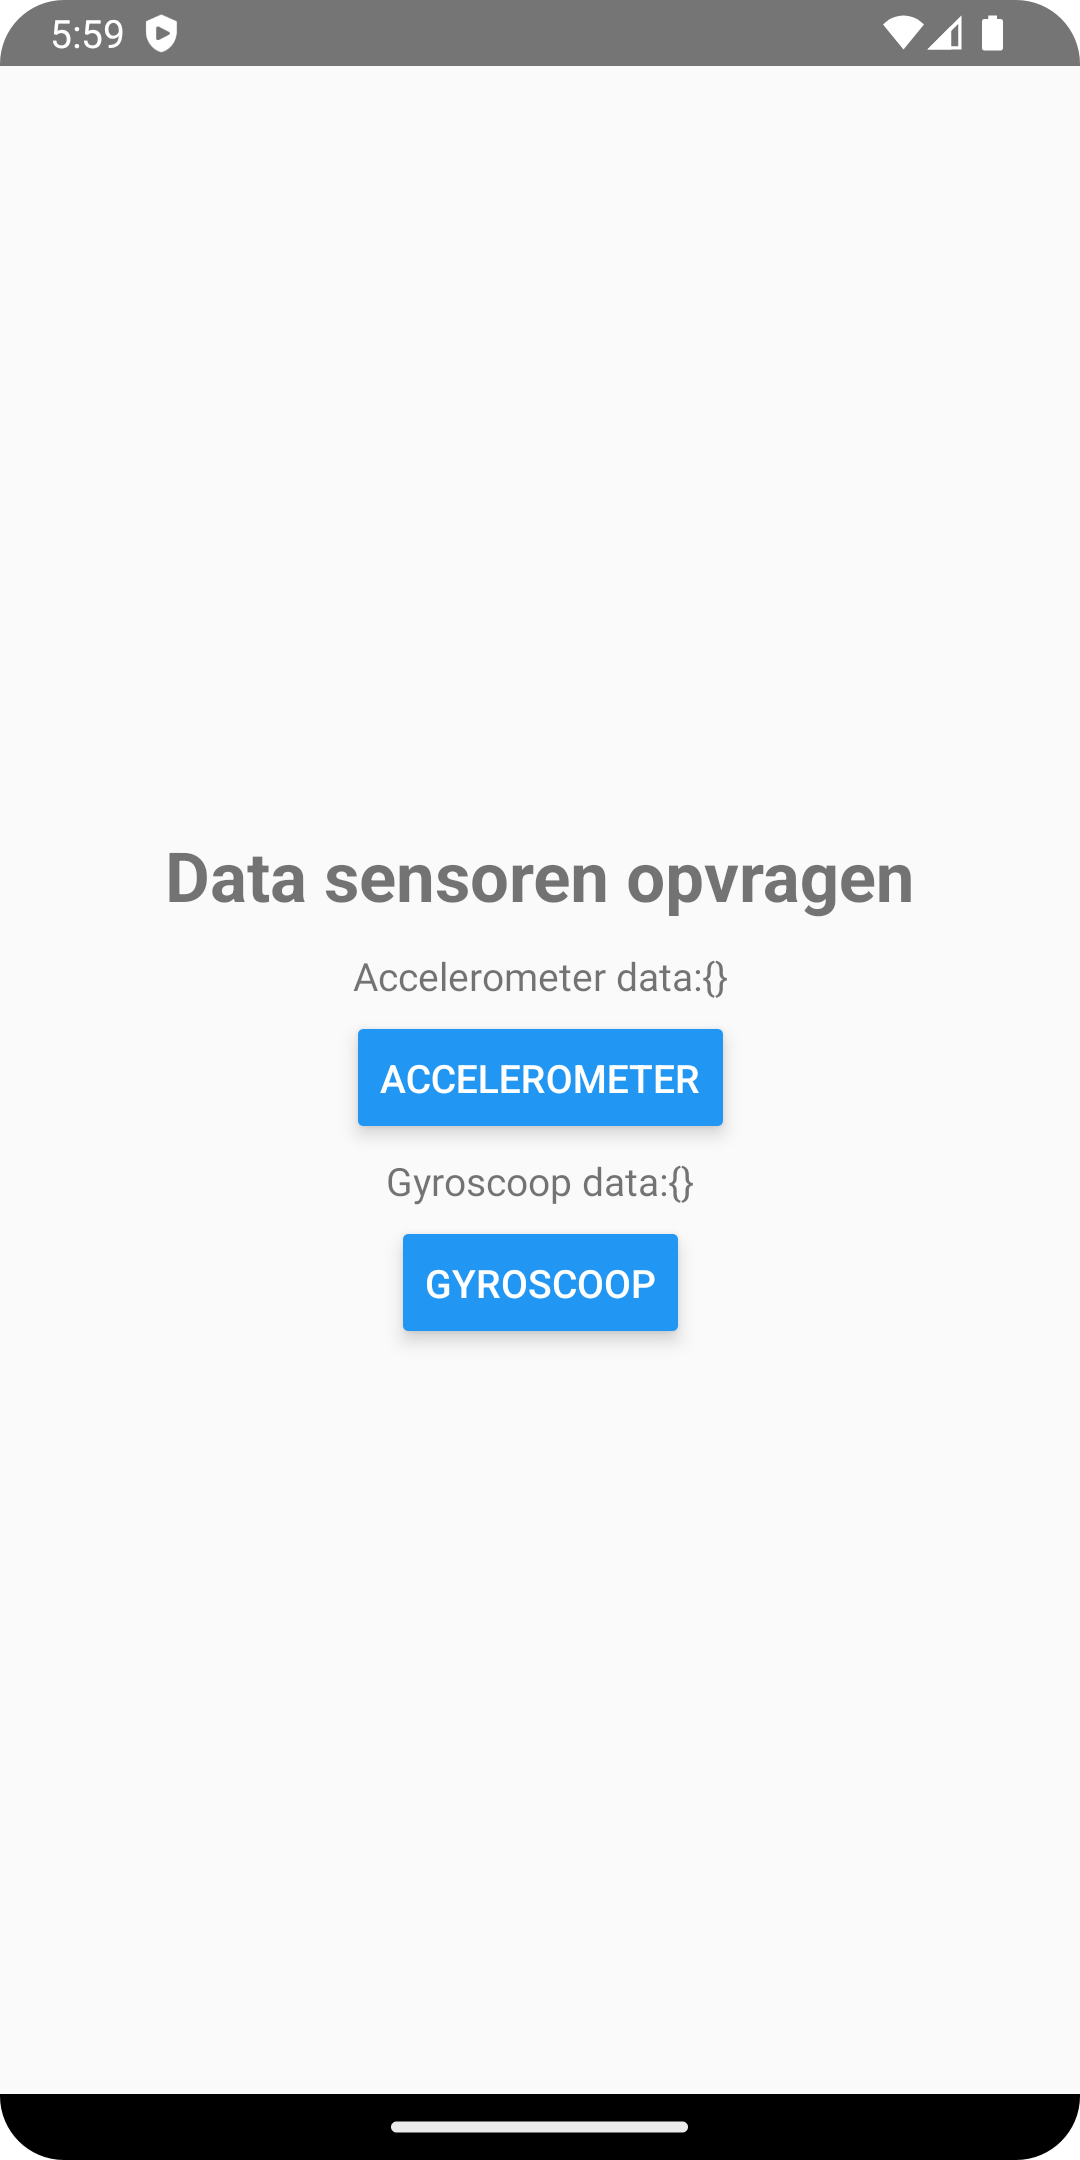
\includegraphics[height=0.4\textheight]{sensoren_layoutcross.png}
    \caption{Layout van applicatie voor data van sensoren op te halen bij React Native.}
\end{figure}
